% !TeX root = relatorio.tex
\documentclass[12pt,a4paper]{article}

\usepackage[T1]{fontenc}
\usepackage[utf8]{inputenc}
\usepackage[brazilian]{babel}
\usepackage{lmodern}
\usepackage[a4paper,margin=2.5cm]{geometry}
\usepackage{amsmath}
\usepackage{amssymb}
\usepackage{graphicx}
% Inclui figura se existir; exibe aviso caso contrário (documento compila sem figuras).
\let\latexincludegraphics\includegraphics
\renewcommand{\includegraphics}[2][]{%
  \edef\@figpath{#2}%
  \IfFileExists{\@figpath}%
    {\latexincludegraphics[#1]{\@figpath}}%
    {\fbox{\footnotesize\itshape figura ausente}}%
}
\usepackage{float}
\usepackage{booktabs}
\usepackage{hyperref}
\usepackage{xcolor}
\usepackage{subcaption}
\usepackage{listings}

\hypersetup{
  colorlinks=true,
  linkcolor=blue,
  urlcolor=blue,
  pdftitle={Relatorio do Trabalho 4},
  pdfauthor={Gustavo Shoiti Sonoda}
}
\urlstyle{tt}

\renewcommand{\contentsname}{Sumário}
\setlength{\parindent}{0pt}
\setlength{\parskip}{0.7em}
\linespread{1.05}

\lstset{
  basicstyle=\ttfamily\footnotesize,
  breaklines=true,
  frame=single,
  columns=fullflexible,
  keepspaces=true,
}

\newcommand{\arquivo}[1]{\nolinkurl{#1}}
\newcommand{\campo}[2]{\textbf{#1.} #2\par}
\newcommand{\figg}[1]{figuras/t4_transformacoes_geometricas/#1}
\newcommand{\figr}[1]{figuras/t4_registro_imagens/#1}

% Grade 2x2 com os quatro interpoladores de uma operação geométrica.
% #1 = stem da imagem, #2 = operacao (ampliacao/reducao/rotacao), #3 = legenda.
\newcommand{\interpquadro}[3]{%
  \begin{figure}[H]
    \centering
    \begin{subfigure}[b]{0.42\textwidth}
      \centering
      \includegraphics[width=\linewidth]{\figg{geo_#1_#2_vizinho.png}}
      \caption{vizinho mais próximo}
    \end{subfigure}\hfill
    \begin{subfigure}[b]{0.42\textwidth}
      \centering
      \includegraphics[width=\linewidth]{\figg{geo_#1_#2_bilinear.png}}
      \caption{bilinear}
    \end{subfigure}

    \vspace{0.6em}
    \begin{subfigure}[b]{0.42\textwidth}
      \centering
      \includegraphics[width=\linewidth]{\figg{geo_#1_#2_bicubica.png}}
      \caption{bicúbica (B-spline)}
    \end{subfigure}\hfill
    \begin{subfigure}[b]{0.42\textwidth}
      \centering
      \includegraphics[width=\linewidth]{\figg{geo_#1_#2_lagrange.png}}
      \caption{Lagrange}
    \end{subfigure}
    \caption{#3}
  \end{figure}%
}

% Imagem original (Parte 1). #1 = stem, #2 = legenda.
\newcommand{\originalfig}[2]{%
  \begin{figure}[H]
    \centering
    \includegraphics[width=0.42\textwidth]{\figg{geo_#1_original.png}}
    \caption{#2}
  \end{figure}%
}

% Par de entrada (Parte 2). #1 = par (foto1...), #2 = legenda.
\newcommand{\parfig}[2]{%
  \begin{figure}[H]
    \centering
    \begin{subfigure}[b]{0.46\textwidth}
      \centering
      \includegraphics[width=\linewidth]{\figr{reg_#1_A.jpg}}
      \caption{imagem A}
    \end{subfigure}\hfill
    \begin{subfigure}[b]{0.46\textwidth}
      \centering
      \includegraphics[width=\linewidth]{\figr{reg_#1_B.jpg}}
      \caption{imagem B}
    \end{subfigure}
    \caption{#2}
  \end{figure}%
}

\begin{document}
\hypersetup{pageanchor=false}
\pagenumbering{gobble}

\begin{titlepage}
  \centering

  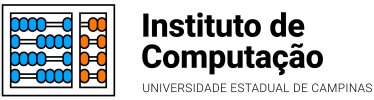
\includegraphics[width=0.24\textwidth]{figuras/logo_ic.png}\par
  \vspace{0.8cm}
  {\large Universidade Estadual de Campinas\par}
  {\large Instituto de Computação\par}

  \vspace{1.5cm}

  {\Large \textbf{Relatório de Implementação do Trabalho 4}\par}
  \vspace{0.5cm}
  {\large Introdução ao Processamento Digital de Imagens (MC920/MO443)\par}
  \vspace{1.2cm}

  {\large Transformações geométricas com interpolação e registro de imagens
    para geração de panoramas.\par}

  \vspace{1.5cm}

  \begin{flushleft}
    \textbf{Professor:} Hélio Pedrini\\
    \textbf{Aluno:} Gustavo Shoiti Sonoda\\
    \textbf{RA:} 217579\\
  \end{flushleft}

  \vfill

  Campinas -- São Paulo\\
  \today
\end{titlepage}

\tableofcontents
\newpage
\hypersetup{pageanchor=true}
\pagenumbering{arabic}

% ===========================================================================
\section{Introdução}
% ===========================================================================

O Trabalho~4 da disciplina MC920/MO443 é dividido em duas partes
complementares. A \textbf{Parte~1} trata de \emph{transformações geométricas}
(escala e rotação) com fatores contínuos, implementando do zero quatro métodos
de interpolação para reamostragem da imagem. A \textbf{Parte~2} trata do
\emph{registro de imagens}: a partir de um par de fotografias parcialmente
sobrepostas, detectam-se pontos de interesse, estabelecem-se correspondências,
estima-se a transformação de perspectiva entre as imagens e gera-se uma imagem
panorâmica.

As duas partes ilustram um contraste metodológico importante. Na Parte~1 o
enunciado proíbe o uso de rotinas prontas de reamostragem: as transformações e
os interpoladores são implementados manualmente a partir das formulações
matemáticas. Já na Parte~2 o enunciado autoriza explicitamente o uso da
biblioteca OpenCV (\texttt{cv2.findHomography}, \texttt{cv2.warpPerspective} e
os detectores de características), de modo que o esforço se concentra na
montagem e na avaliação comparativa do \emph{pipeline} de registro.

Este relatório descreve os algoritmos e as estruturas de dados empregados, as
considerações de implementação, os testes realizados sobre o conjunto de
imagens da disciplina e as limitações observadas.

% ===========================================================================
\section{Materiais e Métodos}
% ===========================================================================

\subsection{Ambiente e organização}

A implementação está em Python~3, organizada no diretório
\arquivo{src/trabalho\_04/} em duas partes:

\begin{itemize}
  \item \arquivo{parte\_01\_transformacoes/} --- com \arquivo{geometria.py}
    (transformações e interpoladores), \arquivo{cli.py} (o programa de linha
    de comando exigido pelo enunciado) e \arquivo{main.py} (geração das
    figuras e dos \emph{benchmarks});
  \item \arquivo{parte\_02\_registro/} --- com \arquivo{panorama.py} (pipeline
    de registro) e \arquivo{main.py}.
\end{itemize}

A infraestrutura compartilhada do repositório (\arquivo{src/common/}) cuida do
\emph{download} e do \emph{cache} das imagens de entrada, da escrita das saídas
e da medição de tempos. As bibliotecas utilizadas são \texttt{NumPy}
(operações vetorizadas), \texttt{Pillow} (E/S de PNG) e
\texttt{opencv-contrib-python} (Parte~2). Os experimentos foram executados em
ambiente Linux.

\subsection{Estruturas de dados}

Na Parte~1, as imagens são representadas como arranjos \texttt{NumPy} de tipo
\texttt{uint8} e forma $(H, W)$ para tons de cinza ou $(H, W, 3)$ para imagens
coloridas. Todos os interpoladores operam de forma idêntica nos dois casos: os
pesos de interpolação são calculados sobre a grade de coordenadas e
multiplicados pelos canais por \emph{broadcasting}. A aritmética intermediária
é feita em ponto flutuante (\texttt{float64}) e o resultado final é arredondado
e recortado ao intervalo $[0, 255]$.

Na Parte~2, as imagens são lidas com o OpenCV no formato BGR. Os pontos de
interesse são objetos \texttt{cv2.KeyPoint}, e os descritores são matrizes
\texttt{NumPy} (de ponto flutuante para SIFT/SURF; binárias para ORB, BRIEF e
AKAZE). A homografia é uma matriz $3 \times 3$.

\subsection{Mapeamento inverso}
\label{sec:mapeamento}

Tanto a escala quanto a rotação são realizadas por \emph{mapeamento inverso}:
para cada pixel $(x', y')$ da imagem de saída, calcula-se a posição
correspondente $(x, y)$ na imagem de entrada e amostra-se essa posição (em
geral não inteira) por interpolação. O mapeamento inverso garante que todos os
pixels da saída sejam preenchidos, evitando os buracos típicos do mapeamento
direto.

Para a escala por um fator contínuo $s > 0$, a posição-fonte é
\begin{equation}
  (x, y) = \left( \frac{x'}{s},\ \frac{y'}{s} \right),
  \label{eq:escala}
\end{equation}
e a saída tem dimensão $\mathrm{round}(s\,H) \times \mathrm{round}(s\,W)$
(ou a dimensão informada pelo usuário).

Para a rotação por um ângulo $\theta$ no sentido anti-horário em torno do
centro $(c_x, c_y)$, o mapeamento inverso aplica a rotação de $-\theta$:
\begin{equation}
  \begin{aligned}
    x &= \cos\theta\,(x' - c_x) - \sin\theta\,(y' - c_y) + c_x, \\
    y &= \sin\theta\,(x' - c_x) + \cos\theta\,(y' - c_y) + c_y.
  \end{aligned}
  \label{eq:rotacao}
\end{equation}
Posições-fonte que caem fora do domínio da imagem de entrada recebem o valor
zero (preto), o que produz os cantos escuros visíveis nas imagens rotacionadas.

% ===========================================================================
\section{Parte 1: Transformações Geométricas}
\label{sec:parte1}
% ===========================================================================

\subsection{Especificação do programa}

Conforme o enunciado, foi implementado um programa de linha de comando que
realiza \emph{uma} transformação geométrica (escala \emph{ou} rotação) por
execução, lendo e gravando imagens em PNG:

\begin{lstlisting}
python3 -m src.trabalho_04.parte_01_transformacoes.cli \
    [-a angulo] [-e escala] [-d largura altura] \
    [-m interpolacao] -i entrada.png -o saida.png
\end{lstlisting}

Os parâmetros são: \texttt{-a} ângulo de rotação em graus (anti-horário);
\texttt{-e} fator de escala; \texttt{-d} dimensão da imagem de saída em pixels;
\texttt{-m} método de interpolação (\texttt{vizinho}, \texttt{bilinear},
\texttt{bicubica} ou \texttt{lagrange}); \texttt{-i} e \texttt{-o} as imagens de
entrada e saída. O programa valida que exatamente uma transformação seja
solicitada por execução.

As subseções seguintes descrevem os quatro interpoladores. Em todas elas,
$x = \lfloor x' \rfloor$ e $y = \lfloor y' \rfloor$ são as partes inteiras da
posição-fonte, e $d_x = x' - x$ e $d_y = y' - y$ as partes fracionárias.

\subsection{Interpolação pelo vizinho mais próximo}

O valor atribuído é o do pixel inteiro mais próximo da posição-fonte. A
formulação por casos do enunciado equivale a arredondar as coordenadas:
\begin{equation}
  f(x', y') = f(\mathrm{round}(x'),\, \mathrm{round}(y')).
  \label{eq:vizinho}
\end{equation}
É o método mais rápido, porém o que mais introduz serrilhado (\emph{aliasing})
e o aspecto ``em blocos'' nas ampliações.

\subsection{Interpolação bilinear}

Usa uma média ponderada pelas distâncias dos quatro vizinhos mais próximos:
\begin{equation}
  \begin{aligned}
    f(x', y') ={}& (1 - d_x)(1 - d_y)\, f(x, y) + d_x (1 - d_y)\, f(x{+}1, y) \\
    &+ (1 - d_x) d_y\, f(x, y{+}1) + d_x d_y\, f(x{+}1, y{+}1).
  \end{aligned}
  \label{eq:bilinear}
\end{equation}
Produz transições suaves a um custo moderado e é um bom compromisso entre
qualidade e desempenho.

\subsection{Interpolação bicúbica (B-spline)}

Utiliza uma vizinhança de $4 \times 4$ pontos, ponderada pelo núcleo B-spline
cúbico:
\begin{equation}
  f(x', y') = \sum_{m=-1}^{2} \sum_{n=-1}^{2}
    f(x{+}m, y{+}n)\, R(m - d_x)\, R(d_y - n),
  \label{eq:bicubica}
\end{equation}
com
\begin{equation}
  R(s) = \frac{1}{6}\Big[ P(s{+}2)^3 - 4P(s{+}1)^3 + 6P(s)^3 - 4P(s{-}1)^3 \Big],
  \qquad
  P(t) = \max(t, 0).
  \label{eq:bspline}
\end{equation}
O núcleo B-spline tem efeito levemente suavizante, atenuando o serrilhado às
custas de uma pequena perda de nitidez.

\subsection{Interpolação por polinômios de Lagrange}

Também emprega uma vizinhança $4 \times 4$, interpolando primeiro ao longo de
$x$ (gerando quatro valores intermediários $L(n)$, um por linha) e depois ao
longo de $y$:
\begin{equation}
  \begin{aligned}
    f(x', y') ={}&
      \frac{-d_y(d_y{-}1)(d_y{-}2)\,L(1)}{6}
    + \frac{(d_y{+}1)(d_y{-}1)(d_y{-}2)\,L(2)}{2} \\
    &+ \frac{-d_y(d_y{+}1)(d_y{-}2)\,L(3)}{2}
    + \frac{d_y(d_y{+}1)(d_y{-}1)\,L(4)}{6},
  \end{aligned}
  \label{eq:lagrange}
\end{equation}
sendo cada $L(n)$, para a linha $y + n - 2$,
\begin{equation*}
  \begin{aligned}
    L(n) ={}&
      \frac{-d_x(d_x{-}1)(d_x{-}2)\,f(x{-}1, y{+}n{-}2)}{6}
    + \frac{(d_x{+}1)(d_x{-}1)(d_x{-}2)\,f(x, y{+}n{-}2)}{2} \\
    &+ \frac{-d_x(d_x{+}1)(d_x{-}2)\,f(x{+}1, y{+}n{-}2)}{2}
    + \frac{d_x(d_x{+}1)(d_x{-}1)\,f(x{+}2, y{+}n{-}2)}{6}.
  \end{aligned}
\end{equation*}
Os resultados são visualmente muito próximos aos da bicúbica, preservando bem
as bordas.

\subsection{Conjunto de teste}

As imagens de teste foram obtidas do diretório de imagens PNG da disciplina e
abrangem conteúdos variados: \emph{baboon} ($512\times512$, colorida, rica em
textura), \emph{butterfly}, \emph{city} e \emph{house} ($512\times512$, em tons
de cinza), \emph{monalisa} ($256\times256$, colorida), \emph{peppers}
($512\times512$, colorida) e \emph{watch} ($1024\times768$, colorida). Para
cada imagem aplicaram-se: ampliação ($s = 1{,}8$), redução ($s = 0{,}4$) e
rotação ($\theta = 30^\circ$), com os quatro interpoladores.

\subsection{Resultados por imagem}

Para cada imagem são apresentados a original, a ampliação e a rotação com os
quatro interpoladores lado a lado. As diferenças entre os métodos são mais
perceptíveis nas bordas e nas regiões de alta frequência, sobretudo na
ampliação.

\subsubsection{baboon}
\originalfig{baboon}{\textit{baboon} --- imagem original ($512\times512$).}
\interpquadro{baboon}{ampliacao}{\textit{baboon} --- ampliação $1{,}8\times$ com os quatro interpoladores.}
\interpquadro{baboon}{rotacao}{\textit{baboon} --- rotação de $30^\circ$ com os quatro interpoladores.}

\subsubsection{butterfly}
\originalfig{butterfly}{\textit{butterfly} --- imagem original.}
\interpquadro{butterfly}{ampliacao}{\textit{butterfly} --- ampliação $1{,}8\times$.}
\interpquadro{butterfly}{rotacao}{\textit{butterfly} --- rotação de $30^\circ$.}

\subsubsection{city}
\originalfig{city}{\textit{city} --- imagem original.}
\interpquadro{city}{ampliacao}{\textit{city} --- ampliação $1{,}8\times$.}
\interpquadro{city}{rotacao}{\textit{city} --- rotação de $30^\circ$.}

\subsubsection{house}
\originalfig{house}{\textit{house} --- imagem original.}
\interpquadro{house}{ampliacao}{\textit{house} --- ampliação $1{,}8\times$.}
\interpquadro{house}{rotacao}{\textit{house} --- rotação de $30^\circ$.}

\subsubsection{monalisa}
\originalfig{monalisa}{\textit{monalisa} --- imagem original ($256\times256$).}
\interpquadro{monalisa}{ampliacao}{\textit{monalisa} --- ampliação $1{,}8\times$.}
\interpquadro{monalisa}{rotacao}{\textit{monalisa} --- rotação de $30^\circ$.}

\subsubsection{peppers}
\originalfig{peppers}{\textit{peppers} --- imagem original.}
\interpquadro{peppers}{ampliacao}{\textit{peppers} --- ampliação $1{,}8\times$.}
\interpquadro{peppers}{rotacao}{\textit{peppers} --- rotação de $30^\circ$.}

\subsubsection{watch}
\originalfig{watch}{\textit{watch} --- imagem original ($1024\times768$).}
\interpquadro{watch}{ampliacao}{\textit{watch} --- ampliação $1{,}8\times$.}
\interpquadro{watch}{rotacao}{\textit{watch} --- rotação de $30^\circ$.}

\subsection{Desempenho dos interpoladores}

A Tabela~\ref{tab:bench-parte1} apresenta os tempos médios de execução dos
quatro interpoladores sobre a imagem \emph{baboon} ($512\times512$, 3~canais),
para a ampliação ($1{,}8\times$) e a rotação ($30^\circ$), com 8~repetições
após 2~execuções de aquecimento. As implementações são totalmente vetorizadas
em \texttt{NumPy}.

\begin{table}[H]
\centering
\caption{Tempos médios de execução por interpolador (\emph{baboon},
  $512\times512\times3$, 8~repetições).}
\label{tab:bench-parte1}
\begin{tabular}{lrr}
\toprule
\textbf{Interpolador} & \textbf{Ampliação $1{,}8\times$ (ms)} & \textbf{Rotação $30^\circ$ (ms)} \\
\midrule
Vizinho mais próximo &   43{,}1 &    8{,}3 \\
Bilinear             &  136{,}0 &   38{,}0 \\
Bicúbica (B-spline)  &  999{,}1 &  266{,}9 \\
Lagrange             &  426{,}2 &  102{,}3 \\
\bottomrule
\end{tabular}
\end{table}

O custo cresce com o tamanho da vizinhança: o vizinho mais próximo usa 1~ponto,
a bilinear 4, e a bicúbica e a Lagrange $4 \times 4 = 16$ pontos cada. A
bicúbica é a mais cara por avaliar o núcleo B-spline (com potências cúbicas)
para os 16~vizinhos; a Lagrange é mais barata por fatorar a interpolação em duas
passagens 1D. A rotação é mais rápida que a ampliação porque mantém o tamanho da
imagem, ao passo que a ampliação $1{,}8\times$ gera uma saída com
$\sim 3{,}2\times$ mais pixels.

\subsection{Discussão}

\campo{Qualidade visual}{Na ampliação, o vizinho mais próximo produz o
característico aspecto ``em blocos'' e bordas serrilhadas, enquanto bilinear,
bicúbica e Lagrange geram transições suaves. Bicúbica e Lagrange preservam um
pouco melhor a nitidez das bordas que a bilinear, com resultados visualmente
quase indistinguíveis entre si.}

\campo{Redução}{Na redução por subamostragem, todos os métodos baseados em
mapeamento inverso amostram apenas uma fração dos pixels originais, o que pode
introduzir \emph{aliasing} quando o conteúdo de alta frequência não é filtrado
previamente. A Figura abaixo ilustra a redução de \emph{baboon}; as diferenças
entre os interpoladores são sutis nesse caso, pois o fator de redução domina o
resultado.}

\interpquadro{baboon}{reducao}{\textit{baboon} --- redução $0{,}4\times$ com os quatro interpoladores.}

\campo{Custo \texttimes\ benefício}{A interpolação bilinear oferece o melhor
equilíbrio para uso geral. Quando a qualidade nas bordas é crítica, a bicúbica
ou a Lagrange são preferíveis; entre as duas, a Lagrange tem custo
computacional menor para qualidade equivalente.}

% ===========================================================================
\section{Parte 2: Registro de Imagens e Panorama}
\label{sec:parte2}
% ===========================================================================

\subsection{Pipeline de registro}

A geração do panorama segue os oito passos do enunciado, implementados em
\arquivo{panorama.py}:

\begin{enumerate}
  \item conversão das imagens de entrada para níveis de cinza;
  \item detecção de pontos de interesse e cálculo de descritores locais;
  \item cálculo das distâncias entre os descritores das duas imagens;
  \item seleção das melhores correspondências (teste de razão de Lowe);
  \item estimativa da homografia por RANSAC (\texttt{cv2.findHomography});
  \item projeção de perspectiva (\texttt{cv2.warpPerspective});
  \item união das imagens alinhadas, formando o panorama;
  \item desenho das retas entre os pontos correspondentes.
\end{enumerate}

\subsection{Detectores e descritores}
\label{sec:detectores}

Foram comparados os detectores/descritores sugeridos no enunciado: \textbf{SIFT}
(\emph{Scale Invariant Feature Transform}), \textbf{SURF} (\emph{Speeded-Up
Robust Features}), \textbf{BRIEF} (\emph{Binary Robust Independent Elementary
Features}) e \textbf{ORB} (\emph{Oriented FAST and Rotated BRIEF}).

SIFT e ORB estão disponíveis no pacote padrão do OpenCV. O BRIEF, que é apenas
um descritor, foi combinado com o detector STAR (ambos do módulo
\texttt{xfeatures2d} do \texttt{opencv-contrib-python}). O \textbf{SURF} é um
algoritmo patenteado (\emph{nonfree}) e não vem compilado nos pacotes
distribuídos via \texttt{pip}; ao instanciá-lo, o OpenCV lança um erro de módulo
\emph{nonfree} indisponível. Por essa limitação prática, o SURF foi mantido na
lista de candidatos mas detectado em tempo de execução como indisponível, e em
seu lugar incluiu-se o \textbf{AKAZE}, um detector/descritor livre e robusto que
representa bem a mesma classe de métodos. O programa verifica automaticamente
quais detectores estão disponíveis no ambiente.

SIFT e SURF produzem descritores de ponto flutuante, comparados pela norma~$L_2$;
ORB, BRIEF e AKAZE produzem descritores binários, comparados pela distância de
Hamming.

\subsection{Casamento e homografia}

O casamento usa o \texttt{BFMatcher} com \texttt{knnMatch} ($k = 2$) seguido do
teste de razão de Lowe: uma correspondência é aceita quando a distância ao
melhor vizinho é inferior a um fator (limiar) vezes a distância ao segundo
melhor --- por padrão, $0{,}75$. As correspondências selecionadas alimentam
\texttt{cv2.findHomography} com RANSAC, que estima a matriz de homografia
$3 \times 3$ e identifica os \emph{inliers}, descartando correspondências
espúrias. O cálculo requer ao menos 4~correspondências.

Estimada a homografia $H$ que leva a imagem B ao referencial de A, calcula-se um
\emph{canvas} que comporta as duas imagens (transformando os cantos de B por
$H$), aplica-se \texttt{cv2.warpPerspective} e sobrepõe-se a imagem A,
compondo o panorama. A título de exemplo, a homografia estimada com SIFT para o
par \emph{foto1} foi
\begin{equation*}
  H_{\text{foto1}} =
  \begin{bmatrix}
     1{,}293 & -0{,}069 & -559{,}57 \\
     0{,}166 &  1{,}224 & -163{,}49 \\
     2{,}77\!\times\!10^{-4} & 3{,}51\!\times\!10^{-5} & 1{,}000
  \end{bmatrix}.
\end{equation*}

\subsection{Resultados por par de imagens}

Para cada par mostram-se as imagens de entrada, as retas de correspondência
(inliers, em verde) e o panorama resultante. Salvo indicação contrária,
correspondências e panorama usam o detector SIFT.

\subsubsection{foto1}
\parfig{foto1}{\textit{foto1} --- par de entrada.}
\begin{figure}[H]
  \centering
  \includegraphics[width=0.95\linewidth]{\figr{reg_foto1_correspondencias_sift.jpg}}
  \caption{\textit{foto1} --- retas de correspondência (SIFT, inliers em verde).}
\end{figure}
\begin{figure}[H]
  \centering
  \includegraphics[width=0.85\linewidth]{\figr{reg_foto1_panorama_sift.jpg}}
  \caption{\textit{foto1} --- panorama (SIFT).}
\end{figure}

\subsubsection{foto2}
\parfig{foto2}{\textit{foto2} --- par de entrada.}
\begin{figure}[H]
  \centering
  \includegraphics[width=0.95\linewidth]{\figr{reg_foto2_correspondencias_sift.jpg}}
  \caption{\textit{foto2} --- retas de correspondência (SIFT, inliers em verde).}
\end{figure}
\begin{figure}[H]
  \centering
  \includegraphics[width=0.85\linewidth]{\figr{reg_foto2_panorama_sift.jpg}}
  \caption{\textit{foto2} --- panorama (SIFT).}
\end{figure}

\subsubsection{foto3}
\parfig{foto3}{\textit{foto3} --- par de entrada.}
\begin{figure}[H]
  \centering
  \includegraphics[width=0.95\linewidth]{\figr{reg_foto3_correspondencias_sift.jpg}}
  \caption{\textit{foto3} --- retas de correspondência (SIFT, inliers em verde).}
\end{figure}
\begin{figure}[H]
  \centering
  \includegraphics[width=0.85\linewidth]{\figr{reg_foto3_panorama_sift.jpg}}
  \caption{\textit{foto3} --- panorama (SIFT).}
\end{figure}

\subsubsection{foto4}
\parfig{foto4}{\textit{foto4} --- par de entrada.}
\begin{figure}[H]
  \centering
  \includegraphics[width=0.95\linewidth]{\figr{reg_foto4_correspondencias_sift.jpg}}
  \caption{\textit{foto4} --- retas de correspondência (SIFT, inliers em verde).}
\end{figure}
\begin{figure}[H]
  \centering
  \includegraphics[width=0.85\linewidth]{\figr{reg_foto4_panorama_sift.jpg}}
  \caption{\textit{foto4} --- panorama (SIFT).}
\end{figure}

\subsubsection{foto5}
O par \emph{foto5} é o mais difícil do conjunto (baixa sobreposição e pouca
textura distintiva). SIFT, BRIEF e AKAZE não obtiveram correspondências
suficientes para uma homografia válida; apenas o ORB conseguiu registrar o par.
Mostram-se, portanto, os resultados com ORB.

\parfig{foto5}{\textit{foto5} --- par de entrada.}
\begin{figure}[H]
  \centering
  \includegraphics[width=0.95\linewidth]{\figr{reg_foto5_correspondencias_orb.jpg}}
  \caption{\textit{foto5} --- retas de correspondência (ORB, inliers em verde).}
\end{figure}
\begin{figure}[H]
  \centering
  \includegraphics[width=0.85\linewidth]{\figr{reg_foto5_panorama_orb.jpg}}
  \caption{\textit{foto5} --- panorama (ORB).}
\end{figure}

\subsection{Comparação entre detectores}

A Tabela~\ref{tab:registro} resume, para cada par e detector, o número de
correspondências aprovadas no teste de razão e o número de \emph{inliers}
identificados pelo RANSAC. A Figura~\ref{fig:foto1-detectores} compara os
panoramas do par \emph{foto1} gerados pelos quatro detectores disponíveis.

\begin{table}[H]
\centering
\caption{Correspondências (\emph{matches}) e \emph{inliers} por par e detector.
  ``---'' indica ausência de homografia válida.}
\label{tab:registro}
\begin{tabular}{llrr}
\toprule
\textbf{Par} & \textbf{Detector} & \textbf{Matches} & \textbf{Inliers} \\
\midrule
foto1 & SIFT  & 1137 & 1091 \\
      & ORB   &  671 &  640 \\
      & BRIEF &  225 &  202 \\
      & AKAZE &  512 &  493 \\
\midrule
foto2 & SIFT  & 2063 & 2038 \\
      & ORB   & 1289 & 1269 \\
      & BRIEF &  197 &  183 \\
      & AKAZE &  819 &  807 \\
\midrule
foto3 & SIFT  &  284 &  273 \\
      & ORB   &  779 &  761 \\
      & BRIEF &   32 &   21 \\
      & AKAZE &  127 &  123 \\
\midrule
foto4 & SIFT  &  358 &  348 \\
      & ORB   &  696 &  688 \\
      & BRIEF &    9 &    4 \\
      & AKAZE &  158 &  153 \\
\midrule
foto5 & ORB   &   43 &   39 \\
      & SIFT  &    5 & --- \\
      & BRIEF &    0 & --- \\
      & AKAZE &    0 & --- \\
\bottomrule
\end{tabular}
\end{table}

A Tabela~\ref{tab:bench-parte2} apresenta o tempo médio de detecção, descrição e
casamento dos dois quadros do par \emph{foto1} ($1000\times667$), com
5~repetições.

\begin{table}[H]
\centering
\caption{Tempo médio de detecção + descrição + casamento por detector
  (\emph{foto1}, $1000\times667$, 5~repetições).}
\label{tab:bench-parte2}
\begin{tabular}{lr}
\toprule
\textbf{Detector} & \textbf{Tempo (ms)} \\
\midrule
SIFT  & 169{,}6 \\
ORB   &  44{,}4 \\
AKAZE &  86{,}5 \\
BRIEF &  22{,}9 \\
SURF  & indisponível (\emph{nonfree}) \\
\bottomrule
\end{tabular}
\end{table}

\begin{figure}[H]
  \centering
  \begin{subfigure}[b]{0.46\textwidth}
    \centering
    \includegraphics[width=\linewidth]{\figr{reg_foto1_panorama_sift.jpg}}
    \caption{SIFT}
  \end{subfigure}\hfill
  \begin{subfigure}[b]{0.46\textwidth}
    \centering
    \includegraphics[width=\linewidth]{\figr{reg_foto1_panorama_orb.jpg}}
    \caption{ORB}
  \end{subfigure}

  \vspace{0.6em}
  \begin{subfigure}[b]{0.46\textwidth}
    \centering
    \includegraphics[width=\linewidth]{\figr{reg_foto1_panorama_brief.jpg}}
    \caption{BRIEF}
  \end{subfigure}\hfill
  \begin{subfigure}[b]{0.46\textwidth}
    \centering
    \includegraphics[width=\linewidth]{\figr{reg_foto1_panorama_akaze.jpg}}
    \caption{AKAZE}
  \end{subfigure}
  \caption{\textit{foto1} --- panoramas gerados pelos quatro detectores
    disponíveis.}
  \label{fig:foto1-detectores}
\end{figure}

\subsection{Discussão e limitações}

\campo{SIFT}{Detecta o maior número de pontos estáveis e produz os casamentos
mais densos e confiáveis, com altíssima taxa de \emph{inliers}, mas é o método
mais lento. É a escolha mais robusta quando o tempo não é crítico.}

\campo{ORB}{Excelente compromisso entre robustez e velocidade. Por ser binário e
rápido, registrou todos os pares --- inclusive o \emph{foto5}, em que os demais
falharam --- sendo a opção mais versátil do conjunto.}

\campo{BRIEF (STAR)}{Gera muito menos pontos e descritores menos distintivos;
funcionou nos pares fáceis, mas degradou rapidamente nos pares com menor
sobreposição (\emph{foto3} e \emph{foto4}) e falhou no \emph{foto5}.}

\campo{AKAZE}{Desempenho intermediário, robusto nos quatro primeiros pares,
servindo como substituto livre adequado ao SURF indisponível.}

\campo{Limitações}{(i)~O SURF não pôde ser avaliado por ser \emph{nonfree} e não
estar disponível nos pacotes \texttt{pip} do OpenCV. (ii)~A união do panorama é
feita por simples sobreposição de A sobre B, sem \emph{blending}, de modo que
diferenças de exposição podem produzir uma costura visível. (iii)~Pares com
baixa sobreposição ou textura pobre (\emph{foto5}) podem não fornecer
correspondências suficientes para alguns detectores. (iv)~As imagens de entrada
muito grandes são redimensionadas para no máximo 1000~pixels no maior lado, para
acelerar o processamento.}

% ===========================================================================
\section{Conclusão}
% ===========================================================================

Na Parte~1, os quatro interpoladores foram implementados do zero a partir das
formulações do enunciado e validados sobre um conjunto variado de imagens. Os
resultados confirmam o comportamento esperado: o vizinho mais próximo é o mais
rápido porém o de menor qualidade; a bilinear é um bom compromisso geral; e a
bicúbica e a Lagrange oferecem a melhor preservação de bordas, a um custo
computacional maior (proporcional ao tamanho da vizinhança $4\times4$). O
programa de linha de comando cumpre a especificação, realizando uma
transformação geométrica por execução em imagens PNG.

Na Parte~2, o \emph{pipeline} completo de registro foi montado com o OpenCV e
avaliado sobre cinco pares de imagens. A comparação entre detectores mostrou que
SIFT entrega as correspondências mais robustas, ORB é o mais versátil e rápido
(único a registrar o par mais difícil), enquanto BRIEF e AKAZE ocupam posições
intermediárias. O SURF não pôde ser avaliado por restrições de licença do
pacote. Os panoramas gerados reproduzem o resultado esperado pelo enunciado,
alinhando corretamente os pares por meio da homografia estimada por RANSAC.

\begin{thebibliography}{9}

\bibitem{gonzalez}
  R.~C.~Gonzalez e R.~E.~Woods.
  \emph{Digital Image Processing}. 4.~ed. Pearson, 2018.

\bibitem{lowe}
  D.~G.~Lowe.
  Distinctive Image Features from Scale-Invariant Keypoints.
  \emph{International Journal of Computer Vision}, 60(2):91--110, 2004.

\bibitem{bay}
  H.~Bay, A.~Ess, T.~Tuytelaars e L.~Van Gool.
  Speeded-Up Robust Features (SURF).
  \emph{Computer Vision and Image Understanding}, 110(3):346--359, 2008.

\bibitem{calonder}
  M.~Calonder, V.~Lepetit, C.~Strecha e P.~Fua.
  BRIEF: Binary Robust Independent Elementary Features.
  \emph{ECCV}, 2010.

\bibitem{rublee}
  E.~Rublee, V.~Rabaud, K.~Konolige e G.~Bradski.
  ORB: An Efficient Alternative to SIFT or SURF.
  \emph{ICCV}, 2011.

\bibitem{opencv}
  G.~Bradski.
  The OpenCV Library.
  \emph{Dr.~Dobb's Journal of Software Tools}, 2000.

\end{thebibliography}

\end{document}
